\chapter[把目标接住：技术安全概念与系统层开发]{把目标接住：\\技术安全概念与系统层开发}

\begin{noteblock}
Semantica 绑定： 本章保存系统开发的推理链与教学案例；唯一机器语义是
\nolinkurl{semantica.chapter_packages.vol2.ch05}，主场景为
\nolinkurl{semantica.vol2.ch05.scenario.primary}。需求/架构本体、CQ、查询、Shape、案例、
规则、oracle、manifest 与 receipt 均在 Semantica，本目录没有可执行替代。
当前为 \nolinkurl{partial}、release \nolinkurl{blocked}；未支持或证据不完整的能力必须保持阻断。
\end{noteblock}

\begin{center}
\vspace{0.2em}
\chapterartfade{%
\adjustbox{max size={0.88\linewidth}{0.27\textheight}}{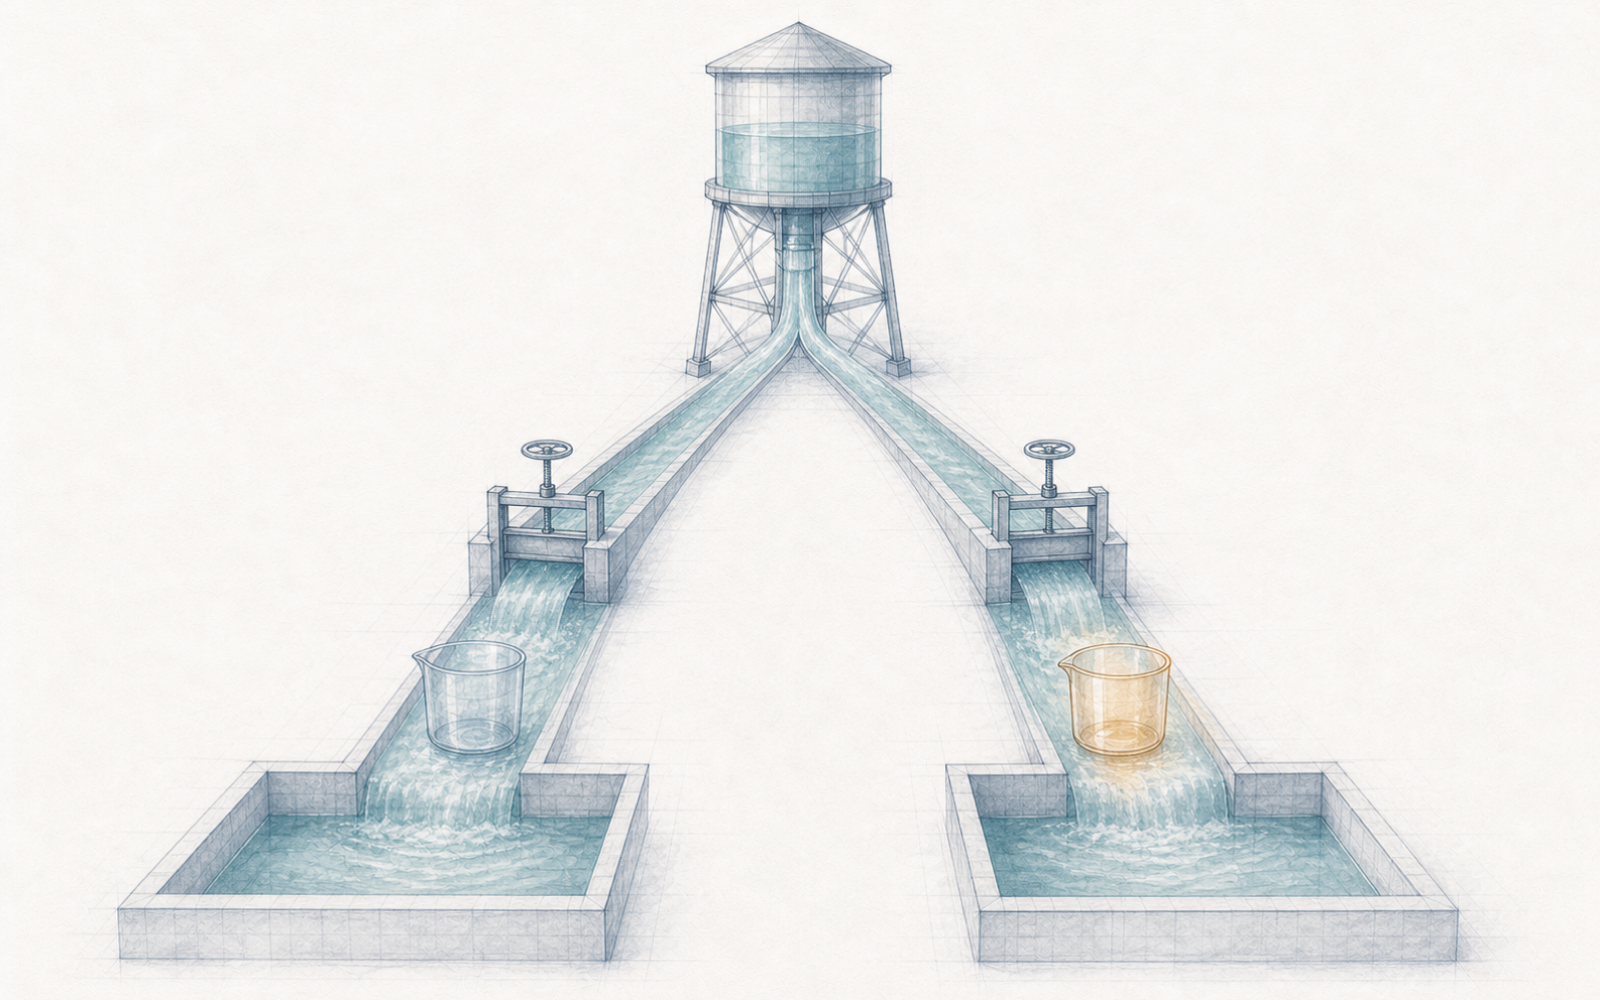
\includegraphics{figures-imagegen/art-ch05-v01.png}}%
}
\vspace{0.35em}
\end{center}

\begin{noteblock}
\textbf{【导读】}
上一章散会时，安全目标和三条候选措施留在了白板上。目标写得再好，它也只是墙上的
一句话——不会自动变成电路、代码、接口和时间预算。本章陪你走完这段落地的全程：
先看一句车辆层的话为什么不能直接发下去执行；再看它被翻译成两级承诺时会丢什么，
承诺拼成架构时要经得起哪些反问；然后停在硬件与软件之间那道最容易没人管的接缝上，
看一场低温试验怎样把一张填得整整齐齐的接口表撕开；接着立起一笔限时的预算，
最后逐层把证据收回来。走到末尾，我们也会诚实地看到：这套纸面做法即使全部做对，
仍有三个地方到不了。
读完本章，你应当能沿着任何一条安全目标向下走到它的每一个承担者，
并在每一次交接处问出：这里丢了什么。
\end{noteblock}

\Needspace{6\baselineskip}
\section{挂在墙上的目标}

周一早上，安全目标被打印出来，贴在项目区的墙上。最重的一条与高速工况的非预期
助力有关：检出之后，必须在危害来得及形成之前让助力受控，或者转入安全状态。
目标旁标着 D——风险语言里最重的一档。有一栏空着：从故障出现到危害可能形成的
容忍窗口，上一章的冻结表格里写的是“待定”，因为它要靠车辆动力学和试验去挣，
不能先抄一个好看的整数。白板的照片也钉在旁边：双信号比较、独立关断、驾驶员告警，
三条候选措施，等着被展开。

陈工把任务交给系统工程师小唐：“分下去。”

怎么分？最省事的做法是把目标原句转发给硬件、软件和供应商，各自“落实”。
这个做法几乎每个项目都试过，它败在一个安静的地方：目标是车辆层的语言。
“非预期助力”对一段代码没有操作含义——软件工程师会按自己的理解设一个偏差阈值，
硬件工程师会按自己的理解做一路限流，两个人都在诚实地落实，两份理解之间的差异
却不会自己暴露，要等到台架或者路上才见面。

那就开个宣贯会，把目标讲透，让大家“心里都有数”？第 2 章已经埋葬过这句话：
默契的覆盖半径只有一张熟人餐桌。何况下周有个新面孔要进项目——转矩传感器供应商
派来的系统工程师梁工，在传感器行业干了十五年，先做应用支持后做系统，
见过太多主机厂把他手册里的脚注当装饰，所以说话总带着前提：“这个值成立的条件是\ldots{}\ldots{}”
他没有参加过任何一次宣贯会，也不欠这个项目任何默契。

原句发不下去，默契靠不住，剩下的只有一条路：一次真正的翻译。
可是，一句车辆层的话，要被翻译成什么，一块电路、一段代码才知道自己该干什么？

\Needspace{6\baselineskip}
\section{翻译，不是抄写}

翻译分两级。第一级仍然站在功能层说话：“检出非预期助力，并在危害形成之前
抑制助力或转入安全状态。”这句话故意不说用几路传感器、在哪颗芯片上比对——
它规定的是功能上要做什么，行话叫\textbf{功能安全需求}。第二级才落到技术上：
“控制器对两路转矩信号做合理性比对，偏差超出受控阈值时，软件请求抑制助力”；
“电机驱动保留一条不依赖主控软件的电流限制通道”。这类在具体层级上给出技术承诺的话，
叫\textbf{技术安全需求}。

两级不是“粗一点”和“细一点”的同一句话，因为承诺的主人换了。一条合格的技术承诺
要能回答一整组问题：什么触发它，系统当时在什么模式，哪个技术主体做出什么反应，
拿什么判成败。模式这一问最容易被省掉：正常行驶中检出偏差，反应是抑制输出、
转入降级；初始化还没完成时检出同样的偏差，反应应当是根本不开启助力；
电流越过硬件限幅时，反应要绕开软件。把三种模式压成一句“异常时采取措施”，
不是简洁，是删掉了三段可以验证的内容。

翻译还要面对安全之外的要求。安全策略希望检出异常后尽快切掉助力，
舒适性要求却希望转矩平滑、不突变——两个都正当，合在一起就是冲突。
这种冲突必须在需求层被显式裁决并留下理由，不能揣着含糊发下去，
留给标定工程师将来在车上凭手感摆平：手感摆平的东西，没有证据，也没有责任人。

还有一件事必须在翻译时想到：安全机制自己也会坏。比对在监视信号，看门狗在监视
软件，限流在监视电流——那么谁在监视它们？一个坏了却长期没人知道的监视者，
等于不存在，而且比不存在更危险，因为所有人都以为它还在。所以自检不是锦上添花，
它的任务是把“坏了但没人知道”的时间压短。两个机制还可能打架：一个要断电，
一个要维持降级供电，同时开口时听谁的——仲裁规则也得是翻译的产物，
不能留给现场随机应变。

两周后，小唐把分配矩阵做完了。每条技术需求都连着上游，每条都有承担者：
控制器、软件、电机驱动、梁工的传感器。覆盖率一栏是百分之百，全绿。
小唐在周会上说了一句让所有人都放松下来的话：\textbf{“每条需求都有主儿了——都接住了。”}

这句话一点都不外行。追溯矩阵是这个行业的通行做法，小唐做得比多数项目认真：
逐条连线，逐条核对，没有一行悬空。如果这样还不算接住，那问题一定藏在
矩阵照不到的地方。

有人提议再加一列“验证方法”，逐条补齐。值得做，但它补的仍是每一行自己的完整性——
矩阵审查的单位是行，而丢失恰恰可以发生在行与行之间：拆分时漏掉的东西
不属于任何一行，加多少列都照不见它。又有人提议让各承担方逐条签收。
也值得做，但每一方认下的是“我认领的这条我能做”，没有人被要求担保
“我们认领的这些条，加起来等于上游那句话”。

撞破它的是梁工。需求评审会上，他第一次到场，听完介绍只问了一个问题：
“我的传感器把故障报出去，要多快，才算够快？”

小唐沿着矩阵找。软件那条写着“检出偏差后请求抑制助力”，在；硬件那条写着
“独立电流限制”，在；传感器那条写着“故障时置诊断位”，也在。可上游那句
“在危害形成之前”——整个目标里唯一的时间条件——拆分之后不在任何一条里。
三个承担者每人领走了一个动作，没有人领走“多快”。矩阵全绿，时间蒸发了。

\textbf{派生不是把一句话越抄越细，而是让承诺换主人；目标不会在换手中自动守恒——每一次交接都要重新清点：触发、模式、动作、判据、时限，少一样，就丢一样。}

顺手多问一层：五样东西里，为什么偏偏是时限最常蒸发？因为拆分是沿着
组织的分工线切的。触发、模式、动作、判据，每一样都能落进某一家的地盘，
认领起来天经地义；“多快”却横跨传感器、软件、电机驱动三家——谁认领它，
谁就得替别人的时延担保。按行认领的制度只给“属于一家的东西”发座位，
于是全链共有的那个条件，成了唯一没有座位的那个。这不是哪个人的疏忽，
是逐行分包这种形式自带的盲区。

顺带把等级说清楚：目标旁那个 D，会沿着派生链一路跟下来。风险等级表达的是
目标被违背的后果有多重，派生只是把同一份责任拆开承包——文档变厚，
不会让风险变轻。想让某一段真正降级，唯一的合法通道是拿出真正独立的冗余
并证明这份独立，那是第 8 章的正题；在此之前，任何悄悄调低的等级都是断链，
不是优化。

现在，每条技术承诺都有了承担者，时限也补进了句子。可承担者们背对背各干各的，
各自正确，拼在一起就自动是一个系统吗？

\Needspace{6\baselineskip}
\section{架构要经得起反问}

架构评审会上，一位新调来的工程师展示了一版更干净的框图：概念阶段的双路
转矩传感器，被改成了单路传感器加软件校验。方框少了一个，成本低了一截，
线条也顺眼多了。

“图更简洁”能不能作为接受理由？不能——简洁描述的是画法，不是论证。
那“老方案评审时大家都没意见”呢？也不能——“没意见”审的往往是图有没有画错，
而不是这样拼为什么就够了。把这两个理由排除掉，真正的问题才露出来：
候选措施里的“双信号比较”，依赖的是两个独立的观察；改成单路之后，
变成了同一份数据被软件看两次。这不是版式优化，是把一项安全策略改没了。

评审会顺着这个口子往下挖，挖出了一个更隐蔽的问题：现有的两路信号
共用一个参考电压。单路漂移时，两路读数拉开差距，比对能抓住；
可如果参考电压漂了，两路读数同向变化，差值依然很小，比对会保持沉默——
恰好在两路同时说谎的时候。“有两路”只是库存，“两路不共享一个能同时欺骗
它们的东西”才是冗余。

评审会还处理了另一个方向的直觉：那条硬件电流限制电路在上一代平台上
用过三代产品，有人主张“老设计，免检”。用过三代确实意味着它携带的未知
毛病更少——这是复用真正的价值；但信任历史不能替新边界体检：供电电压不同、
温度范围不同、失效模式的表现也可能不同。评审会最后既没有删掉它，
也没有盖章放行，而是把它保留为候选，附上一项适用性核对任务——
复用改变的是未知量的起点，不是证据义务的终点。

这场分析的产物不是一份报告，而是三处设计改变：参考电压要么独立供给、
要么被单独监控；软件校验之外保留那条硬件电流限制，作为软件失控时的兜底；
控制器与电机之间预留能观测命令值、实际电流和故障状态的测试点——因为等到
集成时才说“需要注入故障”，就只能拆台架补设计了。可测性不是测试团队的愿望清单，
它是架构自己的属性。

到这里可以把一个容易被改名蒙混的概念说死。一摞技术需求，加一张框图，
再加一份“为什么这样拼就足以兑现这些需求”的理由——三样合在一起，
才叫\textbf{技术安全概念}。把需求清单的文件名改成“概念”，不会让内容多出一克。
而那份理由必须诚实：说得出当前证据支持到哪一步，也说得出还不支持什么。
“分析还没做，所以只能声称结构齐了”不丢人；用形容词把没做的事盖过去才丢人。

\textbf{架构不是需求的收纳盒，而是一份必须经得起反问的论证——“为什么这样拼就够了”。答不上反问的框图，只是画得整齐的愿望。}

架构把活切给了硬件和软件，两边各自开工。可切缝正上方那道线——
硬件交出的信号和软件读走的数据之间——归谁？

\Needspace{6\baselineskip}
\section{接缝上的合同}

接口表有两百多行：信号名、方向、量程、单位、更新周期，填得整整齐齐。
软件负责人小林在例会上说：“接口表都填满了，两边照表干活就行。”
这句话同样不外行——信号表是每个项目都在用的工具，能把两百多行填满核对完，
已经好过一半项目。

冬天来的时候，这张表挨了一记重的。

低温环境试验，零下三十度，台架上的助力时断时续，诊断反复报“两路转矩信号
不一致”。排查用了三天：小林的团队先查自己的滤波和去抖，硬件查线束和接插件，
都没有问题。最后是示波器给出了答案——低温下，一路信号的更新周期明显变长了。
翻开梁工的手册，“更新周期 2 毫秒”旁边有个脚注：典型值；低温补偿运行时，
最坏可达数倍。为什么补偿一开，更新就慢？道理不玄：越冷，芯片里的原始信号
漂得越厉害、毛刺也越多，传感器得先量自己的温度，按温度把读数修一遍，
再多采几次做平均把毛刺压下去，才敢把这个数发出去——每个数出门之前
多干了几道活，更新周期自然被拉长。而“2 毫秒”是常温下量出来的：
常温里这些活几乎不用干，数是顺着直道跑出来的。
接口表誊抄时留下了“2”，丢掉了“典型”两个字和那行条件。
方向盘上的转矩一变，正常那路已经跟上，慢的这路还停在上一个值，
两路的瞬时差被拉开；软件按 2 毫秒设计的比对窗口没给这种滞后留位置，
把一个只是更新慢了的旧值，当成了两路分歧，于是助力被尽职尽责地反复抑制。

没有人说谎：手册是真的，表是认真填的，代码是照表写的。代价却是真的——
当季的低温试验窗口作废，重新排队五周；接口表两百多行逐行补“条件”和“最坏值”
两列，重新会签；梁工和小林各自返工。三份局部正确的工作，又一次拼出了
一个全局错误。

事后的补救提议也熟悉。有人说把两家文档合订成册，互相可见——可见不等于承诺：
手册是供应商对器件的描述，不是对这个项目的担保，合订之后脚注照样可以被忽略。
有人说以后对接会逐行过表——这次事故之前恰恰开过对接会，逐行过的就是那张表；
表的格式里根本没有“什么条件下成立”“最坏什么样”“坏了怎么表现”的位置，
把一张缺列的表过得再认真，也只是把缺陷核对得更整齐。

真正缺的是一份属于接缝自己的合同——把硬件与软件的交互写在同一份受控文件上，
行话叫\textbf{硬件-软件接口}。它比信号表多出的，正是那几列救命的内容：
这个值什么时候开始可信（初始化阶段可能送出格式正确、语义还没生效的数）；
最坏什么样（最坏更新、最坏延迟，而不是典型值）；坏了怎么说（诊断位最晚
什么时候置位、保持多久、谁必须在多长时间里读走它）；共享的资源谁来仲裁。
这份合同要在两边开工之前签——事后从代码和原理图里倒推出来的接口文件，
是对现状的辩护，不是对双方的约束。签了之后它也不能死掉：传感器换代、
轮询放宽，任何一方的“局部小改”都是合同变更，不许被描述成“接口没变”。

\textbf{接缝不属于任何一方，所以必须有自己的合同；合同的要害不是“交什么”，而是“什么条件下成立、最坏什么样、坏了怎么说”。两份各自正确的文档，拼不出一个正确的中间。}

合同里写满了毫秒：更新周期、置位时限、读走窗口。这些数字不是各自随手填的——
它们从哪笔总账里分出来？

\Needspace{6\baselineskip}
\section{一笔限时的预算}

故障发生的那一瞬间，危害通常还没有出现。电机转矩要建立，车辆的响应要发展，
驾驶员的手还来得及做一点校正——从故障出现到危害真正可能形成，中间有一个窗口。
要记住这个窗口属于谁：它属于危害和整车情境，由车辆动力学和使用场景决定，
描述的是“如果没有任何机制出手，最坏多快会出事”。它不属于任何一个安全机制。

机制有自己的钟：从故障发生到被检出是一段，从检出到完成反应、进入安全状态
又是一段，两段加起来，必须小于那个窗口。

面对这道题，第一种自然做法是“把机制做快点，多留余量”。快不是免费的：
更快的检测意味着更短的去抖和判定，也就意味着更多误报——低温那三天的教训，
起点正是一个设得过紧的窗口。余量也不是态度词，它得说得出是多少毫秒、
相对哪一个最坏值。第二种做法更隐蔽：“我们的机制全程需要三百毫秒，
那就把窗口定成三百五。”这是让选手自己挪终点线——窗口由危害动力学决定，
不由机制的方便决定，倒推出来的窗口什么也保护不了。

账要怎么算，用一组纯演示的数字走一遍（它们不是这套转向系统的参数）：
设窗口两百毫秒。诊断每二十毫秒跑一次，连续三次命中才判定故障，
那么最坏情况下——故障刚好发生在一次诊断结束之后——检出要六十毫秒；
反应最坏九十毫秒；合计一百五十，还剩五十毫秒余量。现在只改一件事：
诊断周期放宽到四十毫秒。三次命中让最坏检出变成一百二十毫秒，
合计二百一十——其他什么都没动，全局已经超时。传感器的更新、软件的轮询、
去抖的次数、执行的动作，每一段都在花同一笔钱；谁多花一毫秒，
别人就少一毫秒，而且往往没人通知。

回到墙上那张表：这套系统自己的容忍窗口，此刻仍然写着“待定”。这不是拖延，
是诚实——数字要靠车辆动力学分析和试验去挣，抄来的整数只会让后面所有推理
建立在一个没有来源的地基上。但账本必须现在就立好：窗口一旦定值，
它将被分给谁、每一段的最坏值由谁承诺、写进哪份合同——这些格子先画出来，
数字到位的那天才有处可记。等数字来了再立账本，各段时延早已各自为政。

\textbf{窗口属于危害，不属于机制；时间预算只能从窗口向下分，不能由机制的能力向上凑——而一笔没有账本的预算，谁都可以多花。}

需求、架构、合同、预算，都立起来了。可它们还都是纸上的承诺——
拿什么证明这些承诺真的成立？


\begin{noteblock}
\textbf{读图任务}：对比上下两条总时间窗口，先看检测、反应和余量如何分配，再看检测延长后哪一段被挤出右边界。
\end{noteblock}

\begin{center}
\begin{minipage}{\linewidth}
\centering
\adjustbox{max size={\linewidth}{0.78\textheight}}{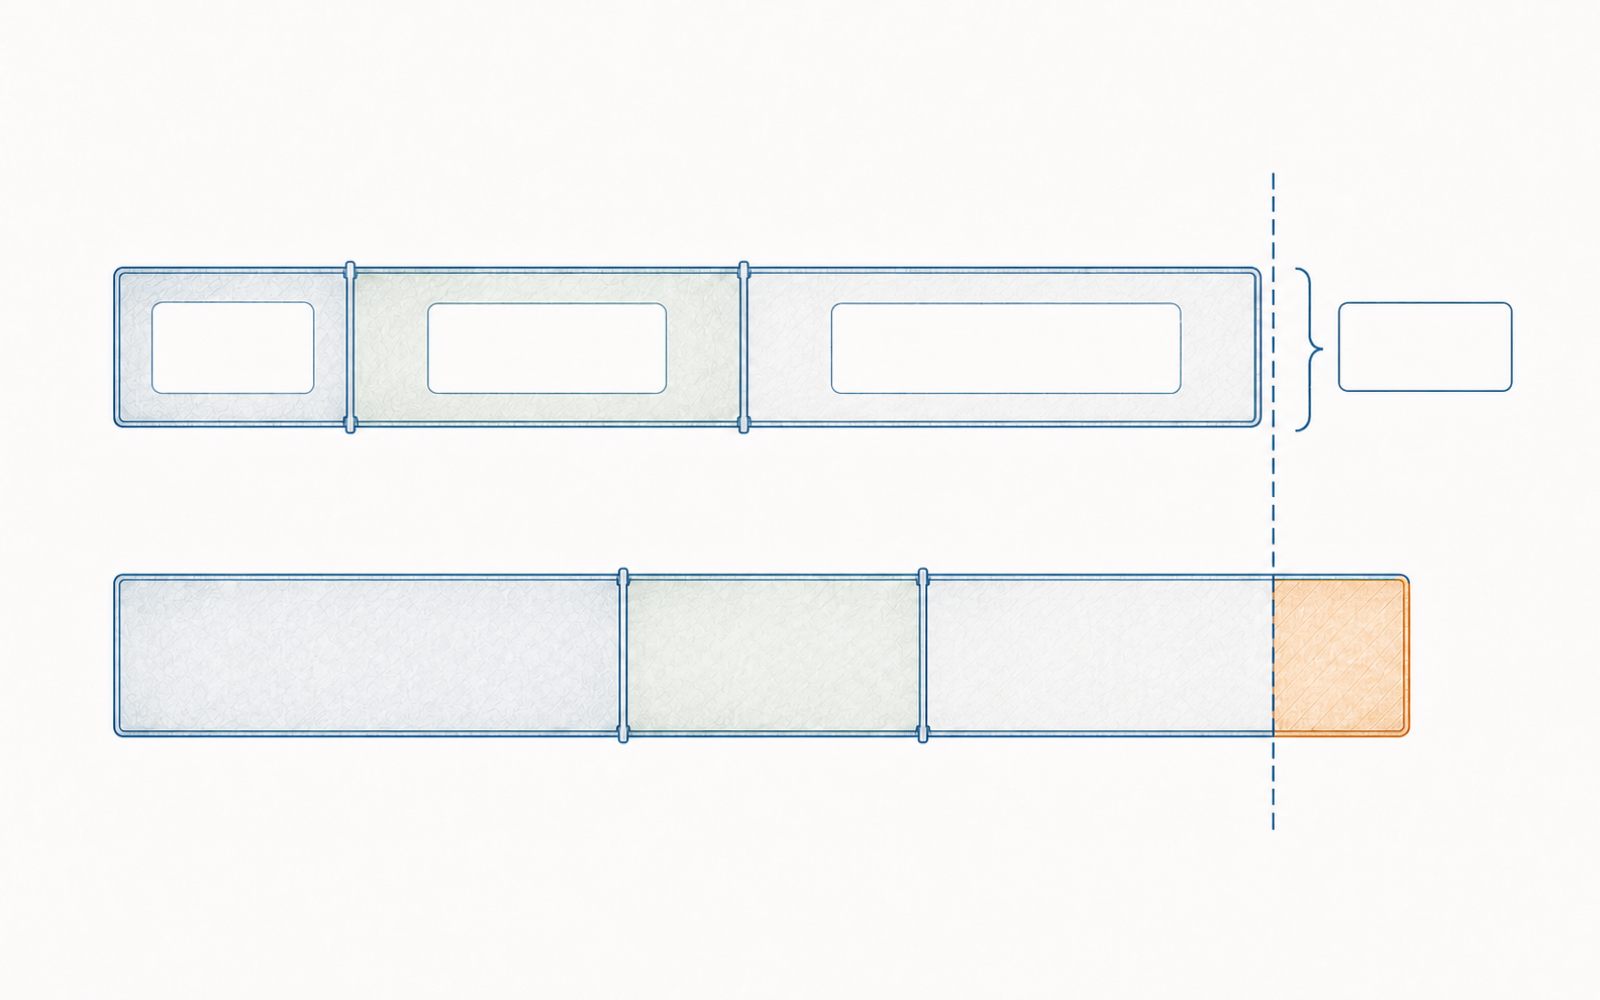
\includegraphics{figures-imagegen/ch05-fig01-time-budget-v01.png}}
\captionof{figure}{系统反应时间是一笔有上限的预算，不是多个团队各自声称足够快就能成立。任一环节超支，都会挤压后续执行和安全余量。}
\end{minipage}
\end{center}


\begin{noteblock}
\textbf{图后判断}：图中的段长是概念性预算，不是某个产品的实测数据。它不单独证明诊断覆盖、反应路径或 FTTI/FHTI 已满足。
\end{noteblock}

\Needspace{6\baselineskip}
\section{逐层收账}

收账的地方在郑工的台架。但集成不是把东西装上车跑一圈，它是三层楼，
每层收的账不一样。

第一层，在元素内部把硬件和软件合到一起，收的是合同的账：诊断位真的在
说定的时间内置位了吗？软件真的在承诺的窗口里读走了吗？低温下的最坏更新
真的落在补签之后的那一格里吗？第二层，把元素合成整套系统，收的是机制之间的账：
比对、限流、告警同时工作时互相打不打架？一个要降级、一个要保持时，
仲裁规则真的裁得动吗？第三层，装进真车，收的是整车的账：故障注入之后，
车辆的轨迹、驾驶员手上的力、与整车电源和通信的相处，是不是都落在判据之内？

同一个故障刺激可以在三层都出现，但问题和判据必须跟着受测对象换。
把同一份测试报告换三个标题，不是三层，是一层刷了三遍漆。郑工还有一条
用教训换来的规矩：下层没关闭的问题，必须显式写进上层的测试清单——
那张“初始化时诊断位偶发误置位”的便签，要么在系统层被验证不会误触发降级，
要么继续往上走，绝不允许躺在下层报告的最后一页里自然死亡。

账收到第三层，还剩一个容易被合并掉的问题。集成测试问的是“我们把东西
做对了吗”——每条写下的需求都兑现了吗。可还有另一个问题：“我们做的
是对的东西吗”——当初那条安全目标，在真实的整车上真的站得住吗？
回答它的活动叫\textbf{安全确认}，它有自己的问题清单：这辆样车凭什么代表
将来卖出去的那一类车？驾驶员真的控制得住吗——包括可以合理预见的误用？
当初危害分析里那些只有到整车上才能检验的假设，逐条评过了吗？
“整车上跑过了”回答不了这些：一辆车不自动等于代表性，跑过不自动等于
按判据收账。想把三层集成和安全确认合并省时间的人，省掉的正是问题本身——
四套问题，四份答案，谁也替不了谁。

\textbf{收账要逐层收，结论不许跳级：每一层的绿灯只在自己那层作数——楼可以一层层上，但没有电梯。}

秋天，账一层层收着，墙上的目标看起来正在稳稳落地。
直到梁工的一封邮件到来。

\Needspace{6\baselineskip}
\section{一张全绿的矩阵，答不上一个问题}

邮件写得很客气：传感器将在下一代改版，制程更替，内部补偿和更新机制都会变；
老款两年后停产，建议项目排查影响。

陈工把邮件转给小唐，只问了一句：“哪些东西要重开？”

小唐有矩阵，有接口合同，有时间账本——这一章立起来的全部家当。他坐下来算，
一个小时后发现自己算不动。第一，矩阵是人手维护的：上季度更新之后，
架构改过两处，接口表补签过一轮，矩阵还不知道——它记录的是上次有人有空时
的世界。第二，矩阵记录的是“这条和那条有关”，不记录“为什么有关、
依赖了它的什么”：比对窗口当年为什么定在那个值？依据的是不是老款传感器的
最坏刷新？这些理由不在矩阵里，只在当年做决定的人的脑子里——
而其中一位已经离职。第三，“哪些要重开”没有任何机械的办法算出来。
最后的解法是把所有相关团队拉进会议室，投影矩阵，逐行认领，开了两天。
散会时清单列了四十多项，没有一个人敢担保它是完整的。

先把公道话说完：这一章走下来的每一步——派生时清点五要素、架构接受反问、
接缝签合同、时间立账本、证据逐层收——都是这个行业用真实事故一条条炼出来的
最佳实践。认真做到这些，已经好过绝大多数团队；这也是没有 AI 的年代，
人类工程共同体能做到的最好水平。

但两天会议暴露的三件事，是这套纸面做法自身的边界，再认真也补不上。
\textbf{其一，追溯靠人手维护，账本的更新永远慢于事实}——矩阵描述的是过去某一天，
而变更发生在今天。\textbf{其二，派生的理由不留痕}——纸面记得住“有关”，
记不住“为什么有关”；可变更影响要问的恰恰是“为什么”：不知道当年为什么
这样拆，就不知道今天要不要重拆。\textbf{其三，影响算不出来}——改一条上游，
没有任何办法可靠地列出下游哪些承诺、哪些判据、哪些试验必须重开，
只能靠会议室、记忆和运气。这不是团队不够认真，是纸面这种载体
记不住这些东西。这三个问题，本章冻结在这里，留给本书的后半部分——
到那里，追溯将不再是一张表，而是一种可以被查问的结构。

会议散场前，另一份清单已经发了出去：系统层给硬件的需求单。上面除了
功能承诺，还有一串数字——每条安全机制被期望达到的失效率量级、
诊断被期望覆盖的比例、留给元器件的那份预算。硬件的同事把单子看了两遍，
在回复邮件里问了一个问题，这个问题要用下一章一整章来回答：

“这串数字，从哪里来？到时候，又拿什么证明我们达到了？”

导读里的承诺，现在可以兑现了。合上书之前，做三件事。
第一，挑出你产品里最高的一条目标，沿着分配一路走到最底层，
在每一次交接处数一数：触发、模式、动作、判据、时限，五样还剩几样——
数字每少一次，你就找到了一次丢失。第二，翻开一张接口表，随便挑一个数字，
问它是典型值还是最坏值、什么条件下成立——如果表里没有地方写答案，
你已经找到了自己的接缝。第三，假装收到一封元件换型邮件，手工列出
下游重开清单，给自己计时，然后问：敢不敢担保没漏？
做完第三件事的那种不踏实，请记住它——本书的后半部分，就从那里开始。


\begin{noteblock}
\textbf{本章注记}：本章的人物、会议、事故经过与全部数字（信号周期、温度、
时间演算、排期、行数等）均为合成教学材料，不对应任何真实企业、真实产品
或真实个人；文中的时间演算仅用于说明预算分摊的一般规律，不是任何实际系统
的参数。正文对功能安全标准内容的转述为自然语言概括，精确表述以标准原文为准；
本章不构成对任何实际系统的需求、架构、接口或测试结论。
\end{noteblock}
